\chapter{Introduzione}

\section{Smart Cities}
Citta intelligenti

\section{Electrical Mobility}

Al giorno d'oggi l'Electrical Mobility (EM) è considerata una degli elementi chiave per ridurre l'inquinamento 
e al contempo liberarsi dalla dipendenza dai combustibili fossili. Questo sta portando a ingenti investimenti
da parte di governi e delle industrie automobilistiche. 

Nel breve periodo il mercato legato all'EM è destinato a crescere rapidamente come  
consuguenza dell'incremento della varietà di Veicoli Elettrici (EVs) introdotti dalle Case Automobilistice. 
Secondo recenti studi infatti il numero di EVs venduti nel periodo tra il 2010 e il 2012 è aumentato del 200\%.
Nonostante il crescente interesse nei confronti dell'EM, recenti analisi di mercato dimostrano
che i benefici ad essa legati saranno tangibili soltanto nel lungo questo è confermato da una ricerca condotta dal 
U.S. National Energy Technology secondo cui il 70\% delle persone non comprerà un EV a causa 
dell'incertezza sulla disponibilità delle stazioni di ricarica. A questo si vanno ad aggiungere le
ben note problematiche riguardanti la capacità, la durata delle batterie e i tempi di ricarica 
estremamente lunghi (nell'ordine delle decine di minuti).

Da un lato la durata dei tempi di ricarica, la limitata capacità delle batterie e la disposizione
degli Electric Vehicle Supply Element influsce direttamente sull'esperienza di guida di ogni autista 
e può avere un impatto decisivo sulla penetrazione di mercato dei veicoli elettrici.
D'altra parte diversi studi hanno dimostrato che l'impatto sulla rete energetica causato dalla
ricarica simultanea di molti Veicoli Elettrici può avere ripercussioni negative e si è 
quindi delineata la necessità di coordinare le attività tra EVs ed EVSEs 

Molti progetti Europei sono stati avviati con lo scopo di limitare queste problematiche. Allo stesso tempo
bisogna considerare che un uno scenario realistico di EM ci sono diverse parti interessate
(es: autisti, case automobilistiche, produttori di energia) coinvolte nella gestione dell'EM.
La ricerca si è mobilitata in direzione dell'Information and Communication Technology (ICT)
per fornire servizi di supporto all'EM e permettere alle parti interessate di cooperare in modo intelligente.
Sebbene siano state sviluppate diverse applicazioni su scenari in piccola scala, si è ancora lontani
dall'ottenere l'interoperabilità tra gli attori in gioco i quali utilizzano diverse tecnologie e dispositivi.

Dato l'elevato costo che avrebbero i test su larga scala, la simulazione costituisce lo strumento più adatto
per testare l'efficenza delle suluzioni ICT prima che vengano realmente sviluppate. Al giorno d'oggi sono stati
sviluppati alcuni simulatori veicolari che permettono un controllo molto fine a livello di veicolo e similarmante
altrettanti modelli di batteria sono stati create al fine di riprodurre in modo realistico le dinamiche di carica e
scarica della batteria.
Tuttavia nessuno di questo strumenti è adatto al fine di studiare le dinamiche assai complesse che si presentano 
nello scenario dell'EM, come l'impatto degli EV sulla rete elettrca cittadina oppure l'effettiva
utilità dell'utilizzo di sistemi di prenotazione delle ricariche. 

Il progetto Internet of Energy (IoE) for Electrical Mobility, il quale è stato fondato dall'Unione Europea
e comprende 40 partner da 10 nazioni Europee, mira a colmare queste lacuna, sviluppando hardware, software 
e sistemi middleware che forniranno un infrastruttura di comunicazione interpolabile tra le parti in gioco
all'interno della (? dire due parole a riguardo smart grid).

Lo scopo di questa tesi, frutto del lavoro congiunto tra UNIBO e ARCES, seguito della tesi di laurea di 
Federico Montori, è fornire contributi su tre diversi fronti a questo progetto. 

Inanzitutto abbiamo sviluppato un architettura software con lo scopo di fornire servizi per l'interazione
tra gi EVs ed EM attraverso lo smartphone. Il servizio centrale è il City Service (CS) il quale
si prende a carico le richieste di ricarica, che arrivano dagli smartphone, fornendo la lista degli EVSEs 
disponibili che piu si adattano alle esigenze dell'utente. Il modello di dati usato dal servizio si basa
su un ontologia che rappresenta tutte le informazioni relative alla smart-grid. Le informazioni sono condivise
attraverso un repository semantico chiamato Semantic Information Broker (SIB), esso garantisce, grazie all'ontologia,
un interazione uniforme tra i vari componenti del sistema.

In secondo luogo abbiamo creato un'applicazione mobile che permette all'utente di monitorare i parametri
della batteria del veicolo e di prenotare slot di tempo presso gli EVSE grazie all'interazione con la 
SIB cittadina. Il servizio di prenotazione da la possibilita di scegliere in base a vari parametri come il prezzo, 
la distanza, il contributo energetico necessario a raggiungere l'EVSE e il tempo totale di ricarica.

Infine abiamo creato una piattaforma di simulazione integrata che permette di valutare su larga scala
l'impatto della EM. Diversamente ad altri tool gia presenti il nostro framework permette di studiare 
il comportamento degli EV, con relativo modello di carica e scariaca della batteria, insieme all'interazione
di essi con la samrt grid attraverso gli EVSE. A questo proposito sono stati usati doversi tool tra i quali
SUMO, un ``simulatore di traffico microscopico``, OMNET++, un simulatore a eventi discreti, e infine per 
far comunicare i due simulatori viene usata l'interfaccia TRACI, messa a disposizione da SUMO, la quale
comunica con OMNET++ attraverso Veins. Grazie a SUMO riusciamo a modellare l'ambiante urbano, nel nostro 
caso Bologna e Torino, includendo dati topografici e altimetrici realistici. OMNET++ invece è stato
utilizzato per implementare i modelli dell'EV, compresa la batteria e il comportamento dell'autista.

\section{Smart-M3}

M3 è un architettura middleware per consentire L'interoperabilità delle informazioni in maniera cross-domain, multi-vendor, multi-device, multi-piattaforma. Smart-M3 è la sua prima implementazione Open Source, proposta da SOFIA, un Progetto Europeo (2009-11), appartenente al framework ARTEMIS. 
La piattaforma implementa il disaccoppiamento tra produttori e consumatori di informazione. In questa architettura tutti gli attori (sensori, dispositivi, servizi, attuatori ecc..) cooperano attraverso un database RDF che è lo standard deciso dal World Wide Web Consortium per la descrizione di informazioni e concetti.

Il Semantic Information Broker (SIB) è l'entità responsabile della conservazione e della gestione delle informazioni condivise nell'architettura M3. Gli agenti Software che si scambiano le informazioni vengono chiamati Knowledge Processors (KPs). L'accesso alla SIB da parte dei KP avviene attraverso lo Smart Space Access Protocol  (SSAP), esso consiste in messaggi XML scambiati attraverso socket TCP/IP. Vengono fornite API che implementano il protocollo SSAP in diversi linguaggi.

L'architettura Smart-M3 permette:

\begin{itemize}
	\item \textbf{Interoperabilità dell'informazione}: L'interoperabilità è resa possibile da un modello di dati condiviso che si basa su tecnologie tipiche del Semantic Web.
	\item \textbf{Notifiche al variare dei dati}: Grazie a un meccanismo di sottoscrizione è possibile ricevere notifiche al variare dei dati specificati.
\end{itemize}

\begin{figure}[H]
	\centering
	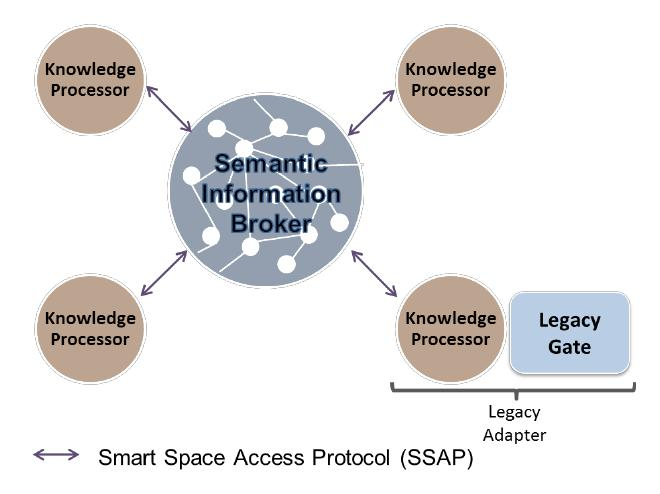
\includegraphics[width=0.5\textwidth]{assets/smart-m3.jpg}
	\caption{Architettura Smart-M3}
	\label{fig:smart-m3}
\end{figure}

\section{Lavori Correlati}

